\documentclass[11pt]{article}
\usepackage[utf8]{inputenc}
\usepackage[ngerman]{babel}

\usepackage{amsmath,amsthm,amssymb,amsfonts}

\usepackage{graphicx}
\graphicspath{{abb/aufgaben-kinematik/}}
\usepackage{float}
\usepackage{tikz}

\usepackage{fancyhdr} % For headers and footers
\usepackage{geometry}
\usepackage{listings}
\usepackage{hyperref}
\hypersetup{
    linkcolor=blue,     
    urlcolor=cyan,
}

\geometry{
    a4paper, % Change this if you intend to print on a different paper size, such as letter paper.
    left=20mm,
    right=20mm,
    top=30mm,
    bottom=30mm,
}

\title{Kinematik - Aufgaben}
\author{Emil Staikov}
\date{}

\begin{document}
\maketitle
\section{Aufgaben aus der IJSO}
\textbf{1.}
\begin{figure}[H]
    \centering
        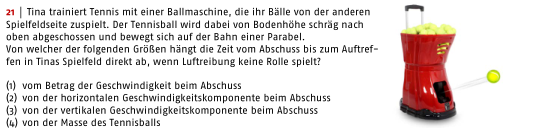
\includegraphics[width=\textwidth]{aufgabe-1.png}
\end{figure} 
\noindent\textbf{2.} 
\begin{figure}[H]
    \centering
        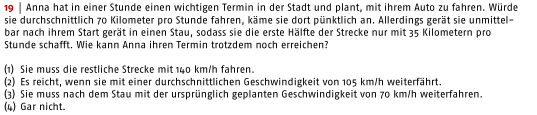
\includegraphics[width=\textwidth]{aufgabe-2.png}
\end{figure} 
\noindent\textbf{3.} 
\begin{figure}[H]
    \centering
        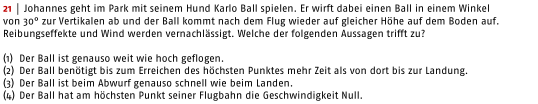
\includegraphics[width=\textwidth]{aufgabe-3.png}
\end{figure} 
\noindent\textbf{4.} 
\begin{figure}[H]
    \centering
        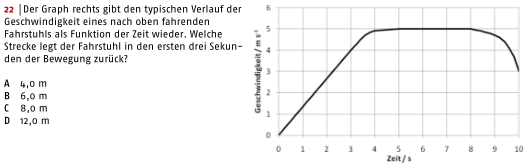
\includegraphics[width=\textwidth]{aufgabe-4.png}
\end{figure} 
\noindent\textbf{5.} 
\begin{figure}[H]
    \centering
        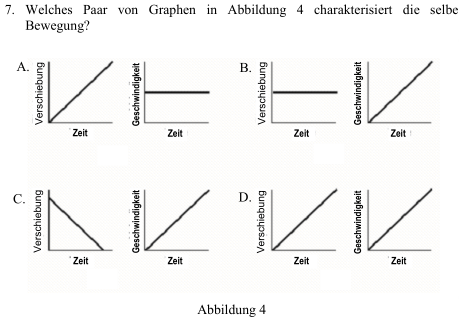
\includegraphics[width=0.7\textwidth]{aufgabe-5.png}
\end{figure} 
\noindent\textbf{6.} 
\begin{figure}[H]
    \centering
        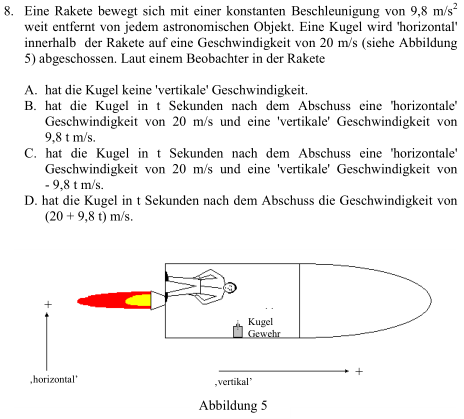
\includegraphics[width=0.7\textwidth]{aufgabe-6.png}
\end{figure} 


\pagebreak

\section{Lösungen}
\textbf{1.} 
\begin{figure}[H]
    \centering
        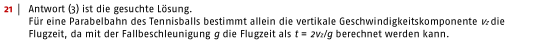
\includegraphics[width=\textwidth]{aufgabe-1-l.png}
\end{figure} 
\noindent\textbf{2.} 
\begin{figure}[H]
    \centering
        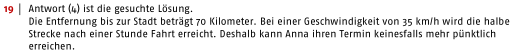
\includegraphics[width=\textwidth]{aufgabe-2-l.png}
\end{figure} 
\noindent\textbf{3.} 
\begin{figure}[H]
    \centering
        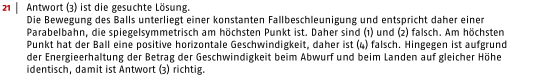
\includegraphics[width=\textwidth]{aufgabe-3-l.png}
\end{figure} 
\noindent\textbf{4.} 
\begin{figure}[H]
    \centering
        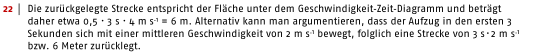
\includegraphics[width=\textwidth]{aufgabe-4-l.png}
\end{figure} 
\noindent\textbf{5.} A. \\\\
\noindent\textbf{6.} C. \\\\

\end{document}